\documentclass{article}
\usepackage{flowchart}
\usepackage{tikz}
\usetikzlibrary{shapes,arrows,chains}
\begin{document}
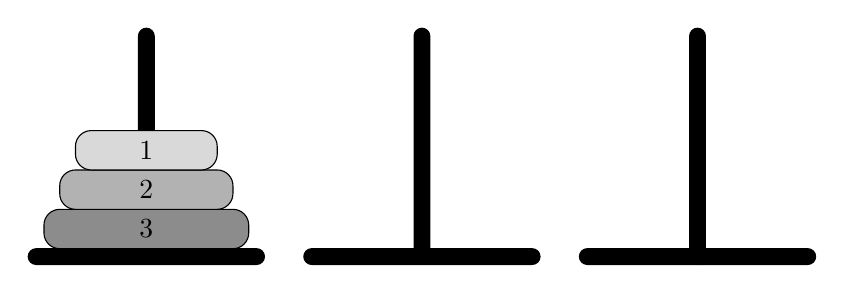
\begin{tikzpicture}[>=latex']
  \draw [rounded corners=.1cm, fill=black] (0,0)--(3cm,0)--(3cm,.2cm)--(0,.2cm)--cycle;
  \draw [rounded corners=.1cm, fill=black] (1.4cm, 0)--(1.4cm,3cm)--(1.6cm,3cm)--(1.6cm,0)--cycle;

  \draw [rounded corners=.2cm,fill=gray!90] (.2cm,.2cm)--(2.8cm,.2cm)--(2.8cm,.7cm)--(.2cm ,.7cm)--cycle;
  \draw [rounded corners=.2cm,fill=gray!60] (.4cm,.7cm)--(2.6cm,.7cm)--(2.6cm,1.2cm)--(.4cm ,1.2cm)--cycle;
  \draw [rounded corners=.2cm,fill=gray!30] (.6cm,1.2cm)--(2.4cm,1.2cm)--(2.4cm,1.7cm)--(.6cm ,1.7cm)--cycle;

  \draw [rounded corners=.1cm, fill=black] (3.5cm,0)--(6.5cm,0)--(6.5cm,.2cm)--(3.5cm,.2cm)--cycle;
  \draw [rounded corners=.1cm, fill=black] (4.9cm, 0)--(4.9cm,3cm)--(5.1cm,3cm)--(5.1cm,0)--cycle;

  \draw [rounded corners=.1cm, fill=black] (7cm,0)--(10cm,0)--(10cm,.2cm)--(7cm,.2cm)--cycle;
  \draw [rounded corners=.1cm, fill=black] (8.4cm, 0)--(8.4cm,3cm)--(8.6cm,3cm)--(8.6cm,0)--cycle;

  \node at(1.5cm,.45cm) {3};
  \node at(1.5cm,.95cm) {2};
  \node at(1.5cm,1.45cm) {1};
\end{tikzpicture}
\end{document}
